\documentclass[]{article}
\usepackage[ ]{indentfirst}
\usepackage{tikz}
\usetikzlibrary{automata, positioning}
\usepackage{booktabs}
\usepackage[ ]{array}
%\usepackage[ ]{amsmath}

\usepackage[ ]{graphicx}
\title{Revisão P2\\Linguagens Formais e Autômatos}
\author{Erickson G. Müller}
\date{}

\begin{document}
\maketitle
\section*{Conteúdos}
	\begin{itemize}
		\item Minimização de AF
		\item Árvores de Derviação
		\item Máquinas Reconhecedoras
	\end{itemize}

\section{Minimização de Autômatos Finitos}
Um autômato finito é mínimo se não possui \textbf{estados inacessíveis, mortos e equivalentes}.\\
Considerando o seguinte AFND, vamos reconhecer esses estados\\
\begin{minipage}[t]{0.43\textwidth}
\centering
\begin{tabular}{|c|c|c|} % Colunas com linhas verticais
            \toprule % Linha superior do booktabs
            & a & b \\
            \midrule % Linha intermediária do booktabs (espaçamento reduzido)
		$\to *A $ & $G$ & $B$\\
		$B$ & $F$ & $E$\\
		$C$ & $C$ & $G$\\
		$*D$ & $A$ & $H$\\
		$E$ & $E$ & $A$\\
		$F$ & $B$ & $C$\\
		$*G$ & $G$ & $F$\\
		$H$ & $H$ & $D$\\
            \bottomrule % Linha inferior do booktabs
        \end{tabular}
\end{minipage} 
\hfill
\begin{minipage}{0.43\textwidth}   
$A\to \{ G,B,F,E,C,A$ \textit{acess}\\
$B\to \{F,E,C,A,B,G$\\
$C\to \{C,G,B,F,E,A$\\
$D \to \{A,H,G,B,F,E,C,D$\\
$E \to \{ E,A,G,B,F,C$\\
$F\to \{ B,C,F,E,A,G$\\
$G\to \{ G,F,B,C,E,A$\\
$H \to \{ H,D,A,C,G,B,F,E$\\
\end{minipage}
    
O algoritmo para encontrar os estados inacessíveis começa com uma lista-chave de todos os estados seguidos dos estados que são possíveis de ser alcançado através daquele. Exemplo $A \to \{ G, B$; Todos os estados que estão à direita compartilham o estados que se podem acessar com o estado à esquerda.

A segunda parte do algoritmo consiste em adicionar esses estados que podem ser acessados em duas transições através dos estados que podem ser acessados diretamente. Exemplo $A \to \{ G, B,F, E$, e assim em ciclo até completar todos os estados.

Por fim, temos que os estados inalcançáveis são $D$ e $H$.

Os estados que são mortos são aqueles que não alcançam, por nenhum fecho transitivo, um estado final. Portanto são os estados

Os estados são equivalentes quando, para cada símbolo, levam ao mesmo tipo de estados. Por exemplo, o $A$ e o $G$ são equivalentes pois $G$ e $G$ são estados finais e $B$ e $F$ são estados não finais.

\begin{minipage}[t]{0.43\textwidth}
\begin{tabular}{|c|c|} % Colunas com linhas verticais
            \toprule % Linha superior do booktabs
            $F$ & $K-F $\\
            \midrule % Linha intermediária do booktabs (espaçamento reduzido)
		$A,G$ & $B,C,E,F$\\
		$[A,G]$ & $[B,C],[C,E]$\\
            \bottomrule % Linha inferior do booktabs
        \end{tabular}
\end{minipage} 
\hfill
\begin{minipage}[t]{0.43\textwidth}
\begin{tabular}{|c|c|c|} % Colunas com linhas verticais
            \toprule % Linha superior do booktabs
             & $a$ & $b$\\
            \midrule % Linha intermediária do booktabs (espaçamento reduzido)
		$\to *[AG]$ & $[AG]$ & $[BF]$\\
		$[BF]$ & $[BF]$ & $[CF]$\\
		$[CE]$ & $[CE]$ & $[AG]$\\
		
            \bottomrule % Linha inferior do booktabs
        \end{tabular}
\end{minipage} 

	\subsection{Exercícios de minimização}
\section{Árvores de Derivação}
	Gramática de operadores:
	$$E::= E+E | E*E | (E)| a$$
	Árvores ilustram o processo de derivação a partir do símbolo inicial para construir uma gramática.
	
	\subsection{Reconhecimento Sintático}
		\begin{itemize}
			\item Ascendente mais à esquerda
			\item Ascendente mais à direita
			\item Descendente mais à esquerda
			\item Descendente mais à direita
		\end{itemize}
		Segue exemplo de uma construção de árvore por abordagem descendente mais à direita para a construção de $a+a*a$. Perceba que a sentença $a+a*a$ pode ser formada pelos nós-folhas da árvore.
		\begin{center}
		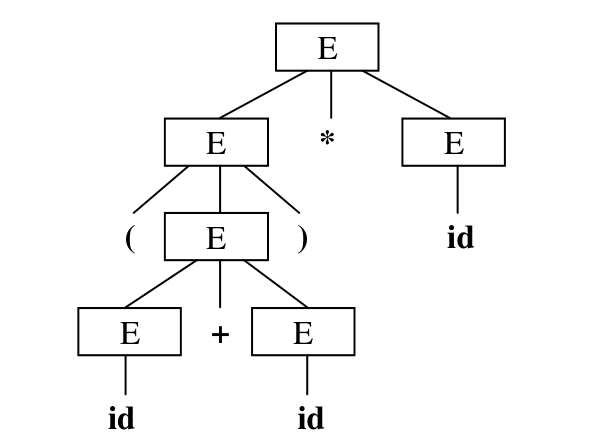
\includegraphics[scale=0.5]{Images/arvore-descendente.png}		
		\end{center}
		
		Em uma abordagem ascendente, a maquina reconhecedora vai identificar qual é a redução que pode ser feita, ao contrário da descendente que verifica a produção por derivação. Por exemplo, na ascendente mais à esquerda começaríamos com a sentença $a+a*a$.  No primeiro símbolos podemos reduzir a produção $a$ em uma produção $E$.
		
		Se uma gramática G tem mais de uma árvore de derivação para uma mesma sentença, então  G é chamada de gramática \textbf{ambígua}. Uma linguagem livre de contexto para a qual toda gramática  livre de contexto é ambígua é denominada linguagem livre de contexto inerentemente ambígua.
		
		A ordem de produções por derivação mais à esquerda é o contrário da ordem de produções por redução mais à direita, e o mesmo se aplica ao contrário.
		
		\newpage		
		\textbf{Exemplo:}
		
		Usando uma gramática de operadores que não é ambígua:
		
		$E::= E+T | T$
% 				1   	2
		
		$T::= T*F | F$
%			   3		4

		$F::= (E)| a$
% 			   5	    6

		
		$$a*(a+ (a*a))$$
		
		Sequência de montagem da árvore.
		\begin{enumerate}
			\item \textbf{Descendente mais à esquerda:} 234651246452346
			\item \textbf{Descendente mais à direita:} 2351452364624646
			\item \textbf{Ascendente mais à esquerda:} 6464264632541532
			\item \textbf{Ascendente mais à direita:} 643254642156432
		\end{enumerate}
		\begin{minipage}[t]{0.43\textwidth}
		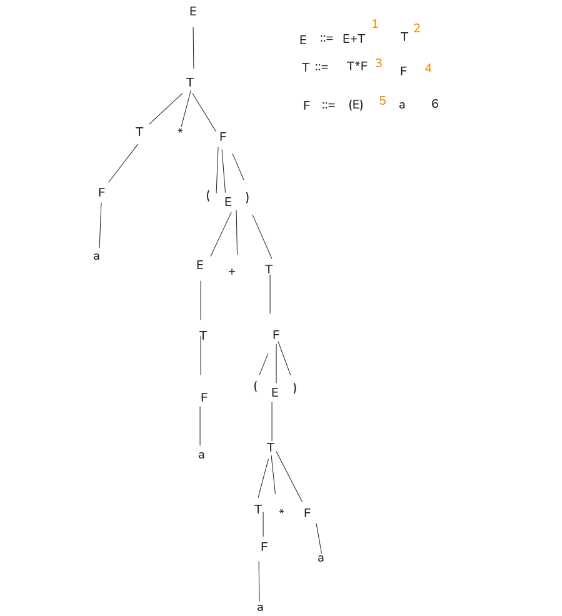
\includegraphics[scale=0.65]{Images/arvore-nao-ambigua.png}
		\end{minipage}
		\hfill
		\begin{minipage}[t]{0.43\textwidth}
		Na ascendente, a árvore fica idêntica apenas com os nós-folhas alinhados no último nível da altura da árvore. Perceba como a sentença $a*(a+(a*a))$ está presente nos nós-folhas dessa árvore.
		\end{minipage}
		\newpage
		
\section{Eliminação de símbolos inúteis (improdutivos e inalcançáveis)}

	$S::= ASB|BSA|SS|aS|\varepsilon$
	
	$A::= ABS | B$
	
	$B::= BSSA|A$
	
	A primeira produção produtiva (que possui apenas símbolos terminais) é o $\varepsilon $, Logo o $S$ é uma produção produtiva. Em seguida vamos marcar todos os símbolos terminais e o não-terminal $S$ em todas as produções. As produções que estão totalmente marcadas ($SS$) são também produtivas.
	
	As produções que não estão totalmente marcadas não são produções produtivas, portanto podem ser descartadas: $ASB, BSA, ABS, B, BSSA, A$. Assim a gramática reduzida é $S::= SS|aS|\varepsilon$
	\\ \\ 
	
	$S::= aS | SB | SS | \varepsilon$
	
	$A::= ASB | c$
	
	$B::= b$
	Marcamos os terminais $\varepsilon, a,c,b$. Percebemos que $S, A, B$ são produções produtivas, portanto podemos marcar todas as produções. Concluindo que não existem produções improdutivas.
	
	\textbf{Exemplo:}
	
	$S::=aSa | FbD$
	
	$D::= Dd |fF|c$
	
	$F::=aA|CA|\varepsilon$
	
	$E ::= BC | eE | EB$
	
	$B ::= bB | FE$
	
	$F ::= fF | Dd$
	
	$C ::= cCb | AcA$
	
	Primeiro passo, marcamos as produções produtivas ($\varepsilon, c$). Percebemos que $D$ e $F$ são produtivos. Em seguida vamos marcar todos os símbolos terminais e os não-terminais produtivos.
	
	\begin{minipage}[t]{0.43\textwidth}
	$S::=\textbf{a}S\textbf{a} | \textbf{F}\textbf{b}\textbf{D}$
	
	$\textbf{D}::= \textbf{D}\textbf{d} |\textbf{f}\textbf{F}|\textbf{c}$
	
	$\textbf{A}::=\textbf{a}\textbf{A}|C\textbf{A}|*\varepsilon*$
	
	$E ::= BC | \textbf{e}E | EB$
	
	$B ::= \textbf{b}B | \textbf{F}E$
	
	$\textbf{F} ::= \textbf{f}\textbf{F} | \textbf{D}\textbf{d}$
	
	$C ::= \textbf{c}\textbf{C}\textbf{b} | \textbf{A}\textbf{c}\textbf{A}$
	\end{minipage}
	
	\hfill
	
	\begin{minipage}[t]{0.43\textwidth}
	$\textbf{S}::=\textbf{a}\textbf{S}\textbf{a} | \textbf{F}\textbf{b}\textbf{D}$
	
	$\textbf{D}::= \textbf{D}\textbf{d} |\textbf{f}\textbf{F}|\textbf{c}$
	
	$\textbf{A}::=\textbf{a}\textbf{A}|C\textbf{A}|*\varepsilon*$
	
	$E ::= BC | \textbf{e}E | EB$
	
	$B ::= \textbf{b}B | \textbf{F}E$
	
	$\textbf{F} ::= \textbf{f}\textbf{F} | \textbf{D}\textbf{d}$
	
	$\textbf{C} ::= \textbf{c}\textbf{Cb} | \textbf{A}\textbf{c}\textbf{A}$
	\end{minipage}
	
	Logo, $E$ e $B$ não são produtivos.
	
		$\textbf{S}::=\textbf{a}\textbf{S}\textbf{a} | \textbf{F}\textbf{b}\textbf{D}$
	
	$\textbf{D}::= \textbf{D}\textbf{d} |\textbf{f}\textbf{F}|\textbf{c}$
	
	$\textbf{A}::=\textbf{a}\textbf{A}|C\textbf{A}|*\varepsilon*$
	
	$\textbf{F} ::= \textbf{f}\textbf{F} | \textbf{D}\textbf{d}$
	
	$\textbf{C} ::= \textbf{c}\textbf{Cb} | \textbf{A}\textbf{c}\textbf{A}$
	
	Agora resta-nos encontrar os alcançáveis.
	
	$S\to \{ S,F,D$
	
	$D\to \{ D, F$
	
	$A \to \{ A,C$
	
	$F \to \{ F,D$
	
	$C \to \{C, A$
	
	Assim S, F e D são as únicas que têm produções alcancáveis e produtivas,
	
			$\textbf{S}::=\textbf{a}\textbf{S}\textbf{a} | \textbf{F}\textbf{b}\textbf{D}$
	
	$\textbf{D}::= \textbf{D}\textbf{d} |\textbf{f}\textbf{F}|\textbf{c}$
	
	$\textbf{F} ::= \textbf{f}\textbf{F} | \textbf{D}\textbf{d}$
	
\section{Fatoração}
	Eliminamos primeiro os indeterminismos diretos para depois eliminar os indeterminismos indiretos.
	
	Uma GLC está  fatorada se ela é determinística, ou seja, se ela não possui produções para  um mesmo não-terminal no lado esquerdo cujo lado direito inicie com a mesma cadeia de símbolos  ou com símbolos que derivam seqüências que iniciem com a mesma cadeia de símbolos. De acordo  com esta definição, a seguinte gramática é não-determinística:  

	$S::= AC | BC$
	
	$A::= aD |cC$
	
	$B::= aB|dD$
	
	$C::= eC | eA$
	
	$D::= fD|AB$
	
	Fatorando o C:
		
	$S::= AC | BC$
	
	$A::= aD |cC$
	
	$B::= aB|dD$
	
	$\textbf{C::= eC'}$
	
	$\textbf{C'::= C|A}$
	
	$D::= fD|AB$
	
	Dá pra fatorar também a produção S, pois começam com não terminal (não-determinismo indireto):

	1º Passo:
		
	$S::= \textbf{aD}C| \textbf{cC}C | \textbf{aB}C | \textbf{dD}C$
	
	$C::= eC'$
	
	$C'::= C | A$
	
	$D::= fD|AB$
	
	2º passo:
	
	$S::= aS' | cCC | dDC$
	
	$S'::= DC | BC$	
	
	Exemplo:
	
	$S:= Abc | bBC | bCD$
	
	$A::= aBC |aDC$
	
	$B::=dCc|dc$
	
	$C::= Acd |dc$
	
	$D::= aBC | abc | aC$

	Mudamos a produção $S$, $A$, $B$ e $D$:
	
	$S::= Abc | bS'$

	$S'::=BC | CD$	
	
	$A ::= aA'$
	
	$A'::= BC |DC$
	
	$B::= dB'$
	
	$B'::=Cc|c$
	
	$C::= Acd |dc$
	
	$D::= aD'$
	
	$D'::= BC | bc | C$
	
	Agora retiramos o não-determinismo indireto:

	$S::= Abc | bS'$

	$S'::=dB'C | AcdD | dcD$	
	
	$A ::= aA'$
	
	$A'::= BC |DC$
	
	$B::= dB'$
	
	$B'::=Cc|c$
	
	$C::= Acd |dc$
	
	$D::= aD'$
	
	$D'::= BC | bc | C$
		
	2° passo:
	
	$S::= Abc | bS'$

	$S'::=dS'' | AcdD$	
	
	$S''::= B'C | cD$
	
	$A ::= aA'$
	
	$A'::= BC |DC$
	
	$B::= dB'$
	
	$B'::=Cc|c$
	
	$C::= Acd |dc$
	
	$D::= aD'$
	
	Substituimos o D:
	
	$S::= Abc | bS'$

	$S'::=dS'' | AcdD$	
	
	$S''::= B'C | cD$
	
	$A ::= aA'$
	
	$A'::= BC |DC$
	
	$B::= dB'$
	
	$B'::=Cc|c$
	
	$C::= Acd |dc$
	
	$D::= aD'$
	
	$D'::= dB'C | bc | Acd | dc$
	
	Novamente:
	
	$S::= Abc | bS'$

	$S'::=dS'' | AcdD$	
	
	$S''::= B'C | cD$
	
	$A ::= aA'$
	
	$A'::= BC |DC$
	
	$B::= dB'$
	
	$B'::=Cc|c$
	
	$C::= Acd |dc$
	
	$D::= aD'$
	
	$D'::= dD'' | bc | Acd$
	
	$D''::= B'C | c$
	
	Produções B e S podem começar com c e podem ser fatoradas mais ainda.
	
\section{Recursão à esquerda}

	Acontece quando uma produção possui uma regra que começa com um não-terminal que é o próprio símbolo da produção

	Ex:
	$$S::= Aab|Bc| ScAB$$	
	$$A::= SAc | BaA |ab$$
	$$B::= Ac |aBb |ab$$
	
	Para eliminar essa recursão à esquerda, mantendo a gramática com a mesma capacidade gerativa. Começamos com a produção que não é recursiva (como $Bc$), e criamos uma nova produção $S'$:
	
	$$S::= AabS' | BcS'$$
	$$S'::= cAbS' | \varepsilon$$
	
	Substituímos as produções que possuem S pelas produções de S' (em A):
	$$A::=AabS'Ac | BcS'Ac | BaA |ab$$
	
	Agora podemos eliminar a recursão à esquerda de A:
	
	$$A::= BcS'AcA' | BaAA' | abA'$$
	$$A'::- abS'AcA' | \varepsilon$$
	
	Não sei o que é isso:
	
	$B::= \textbf{B}cS'AcA'c|\textbf{B}aA'Ac | abAc | aBb | ab$ \textit{Professor riscou essa produção}
	
	$B::= abAcB' | aBbB' |abB'$
	
	$B'::= cS'AcA'cB' | aAA'cB'|\varepsilon$
	
\textbf{	Exemplo:}
	
	$S::= SaB | Sbc | Acd$
	
	$A::= ABc | Acd | Bcd | Cd$
	
	$B::= Acd | Bcc | Cde$
	
	$C::= Ac | Cd | dc$
	
\textbf{	Primeiro em S:}
	
	$S::= AcdS'$
	
	$S'::= aBS' | bcS' | AcdS' | \varepsilon$
		
	$A::= ABc | Acd | Bcd | Cd$
	
	$B::= Acd | Bcc | Cde$
	
	$C::= Ac | Cd | dc$
	
\textbf{	Agora em A:}
	
	$S::= AcS'$
	
	$S'::= aBS' | bcS' | AcdS' | \varepsilon$
	
	$A::= BcdA' | CdA'$
	
	$A'::= BcA' | cdA' | \varepsilon$
	
	$B::= Acd | Bcc | Cde$
	
	$C::= Ac | Cd | dc$
	
\textbf{	Agora em B:}
	
	$S::= AcS'$
	
	$S'::= aBS' | bcS' | AcdS' | \varepsilon$
	
	$A::= BcdA' | CdA'$
	
	$A'::= BcA' | cdA' | \varepsilon$
	
	$B::= AcdB' | CdeB'$
	
	$B'::= ccB' | \varepsilon$
	
	$C::= Ac | Cd | dc$
	
\textbf{	Agora em C:}

	$S::= AcS'$
	
	$S'::= aBS' | bcS' | AcdS' | \varepsilon$
	
	$A::= BcdA' | CdA'$
	
	$A'::= BcA' | cdA' | \varepsilon$
	
	$B::= AcdB' | CdeB'$
	
	$B'::= ccB' | \varepsilon$
	
	$C::= AcC' | dcC'$
	
	$C'::= dC' | \varepsilon$
	
\end{document}
